% Generated by scripts/convert_report.py from source/report.md.


\FloatBarrier

\Needspace{6\baselineskip}

\section{THỰC NGHIỆM VÀ ĐÁNH GIÁ KẾT QUẢ}


Chương này trình bày kết quả kiểm chứng nền tảng MLOps được triển khai trên AWS, tập trung vào khả năng vận hành hạ tầng, huấn luyện và quản lý mô hình, cung cấp dịch vụ suy luận, giám sát hiệu năng và kiểm soát quá trình phát hành. Các thí nghiệm được thực hiện trên hệ thống thực tế và đối chiếu thông qua giao diện quản lý, kết quả API, GitHub Actions và dữ liệu giám sát.


\FloatBarrier

\subsection{Kiểm chứng hạ tầng triển khai trên AWS}


Hệ thống đã được triển khai thành công trên Amazon EKS tại khu vực \code{ap-southeast-1}, sử dụng Kubernetes phiên bản 1.36. Cluster \code{mlops-aws-dev} hoạt động ở trạng thái \textbf{Active}, với ba worker nodes thuộc hai nhóm tài nguyên: hai node phục vụ các thành phần hệ thống và một node dành cho dịch vụ suy luận.


Các node sử dụng EC2 \code{t3.large} On-Demand, trong khi tài nguyên huấn luyện được cấp phát động thông qua Karpenter trên Spot Instances. Quá trình kiểm thử ghi nhận Training Jobs thực thi thành công trên các Spot nodes và các tài nguyên tạm được thu hồi sau khi hoàn tất.


\begin{figure}[!htbp]
\centering
\begin{subfigure}{\linewidth}
\centering
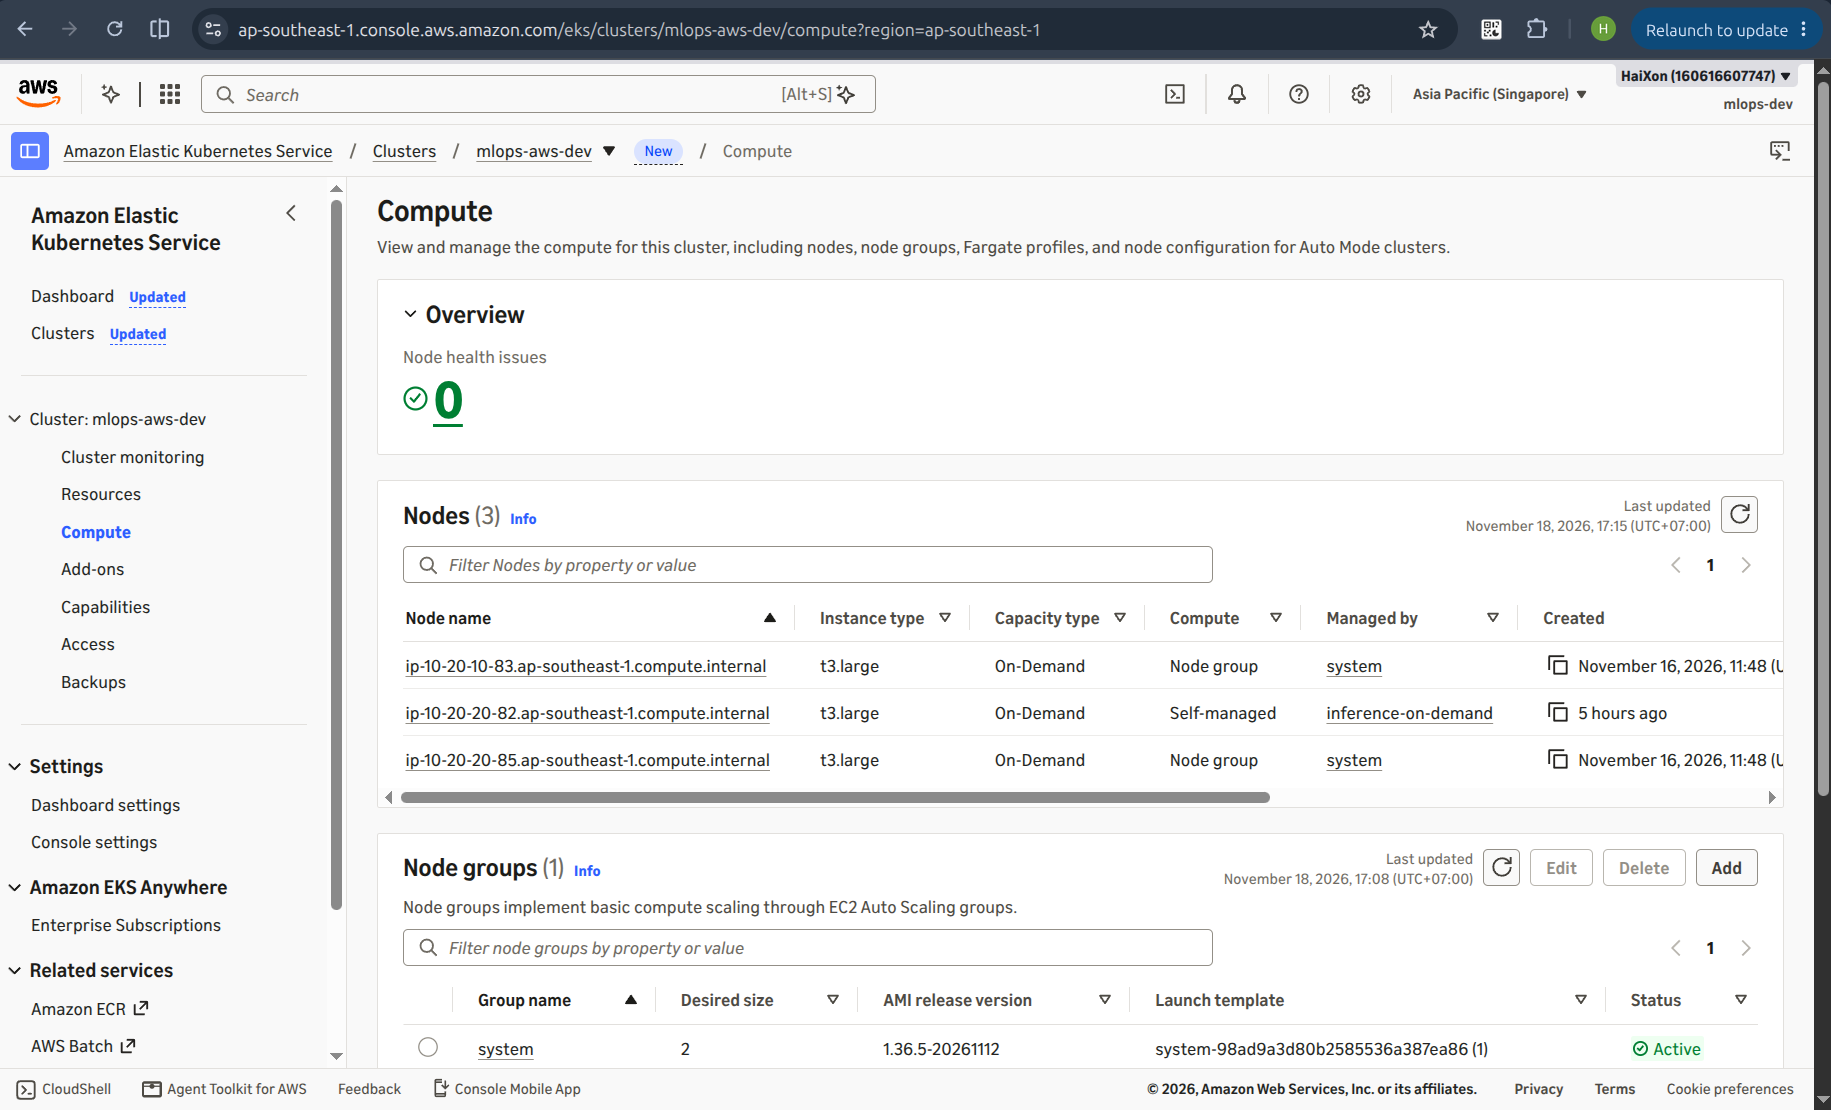
\includegraphics[width=0.94\linewidth,height=0.30\textheight,keepaspectratio,trim={365.00000bp 35.00000bp 30.00000bp 475.00000bp},clip]{Pictures/h01-nodes.png}
\caption{Các worker nodes}
\end{subfigure}\par\medskip
\begin{subfigure}{\linewidth}
\centering
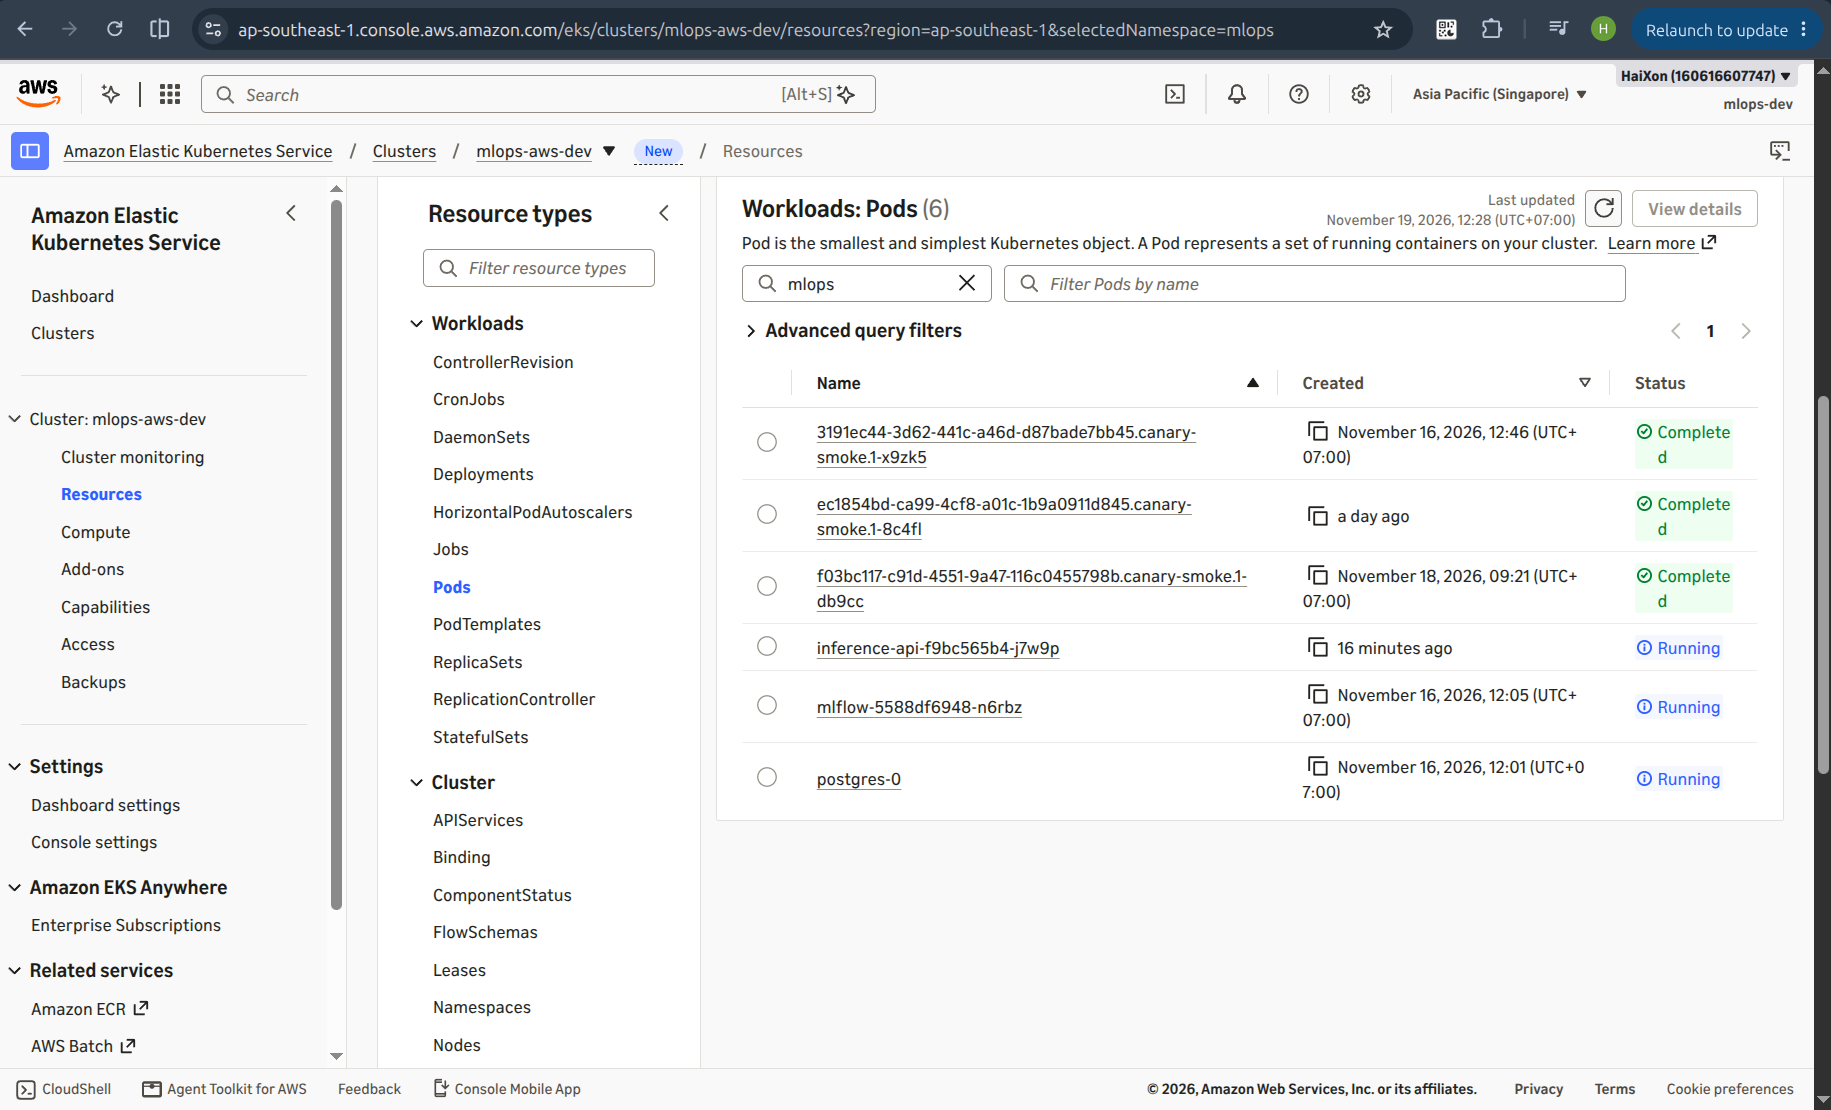
\includegraphics[width=0.94\linewidth,height=0.30\textheight,keepaspectratio,trim={715.00000bp 285.00000bp 40.00000bp 175.00000bp},clip]{Pictures/h01-workloads.png}
\caption{Các workloads trong namespace mlops}
\end{subfigure}\par\medskip
\caption{Hạ tầng tính toán và các workloads đang hoạt động trên Amazon EKS.}
\label{fig:h01}
\end{figure}

Tại namespace \code{mlops}, các thành phần chính gồm PostgreSQL, MLflow và FastAPI inference đều hoạt động ở trạng thái Running. Kết quả này xác nhận các dịch vụ của nền tảng đã được triển khai và vận hành trên hạ tầng AWS thay vì chỉ được kiểm chứng trong môi trường phát triển cục bộ.


\FloatBarrier

\subsection{Đánh giá quá trình huấn luyện và quản lý mô hình}


\subsubsection{Kiểm chứng Model Validation Gate}


Nhóm thực hiện hai trường hợp huấn luyện nhằm kiểm chứng khả năng chấp nhận hoặc từ chối mô hình mới. Các thí nghiệm sử dụng cùng tập dữ liệu đánh giá và duy trì ngưỡng yêu cầu cải thiện tối thiểu \textbf{1\% Validation MAE} so với mô hình champion hiện tại.


\begin{figure}[!htbp]
\centering
\begin{subfigure}{\linewidth}
\centering
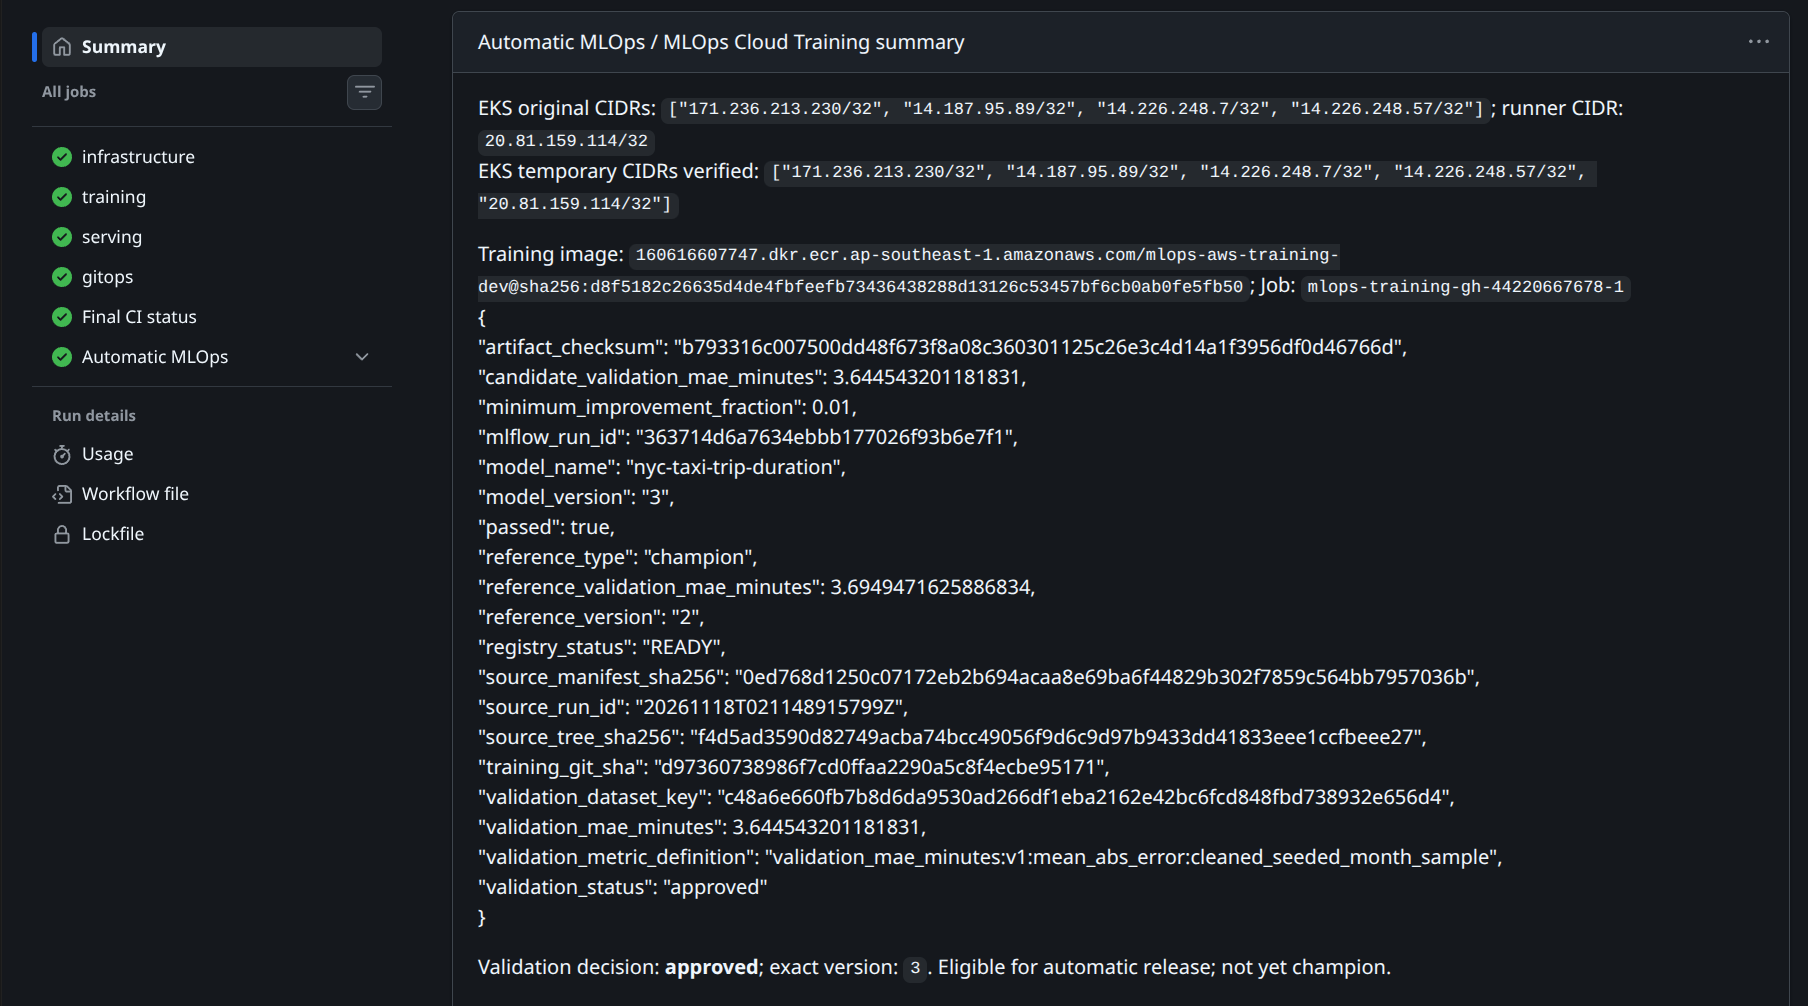
\includegraphics[width=0.94\linewidth,height=0.30\textheight,keepaspectratio,trim={450.00000bp 0.00000bp 10.00000bp 300.00000bp},clip]{Pictures/h02-approved.png}
\caption{Candidate được phê duyệt}
\end{subfigure}\par\medskip
\begin{subfigure}{\linewidth}
\centering
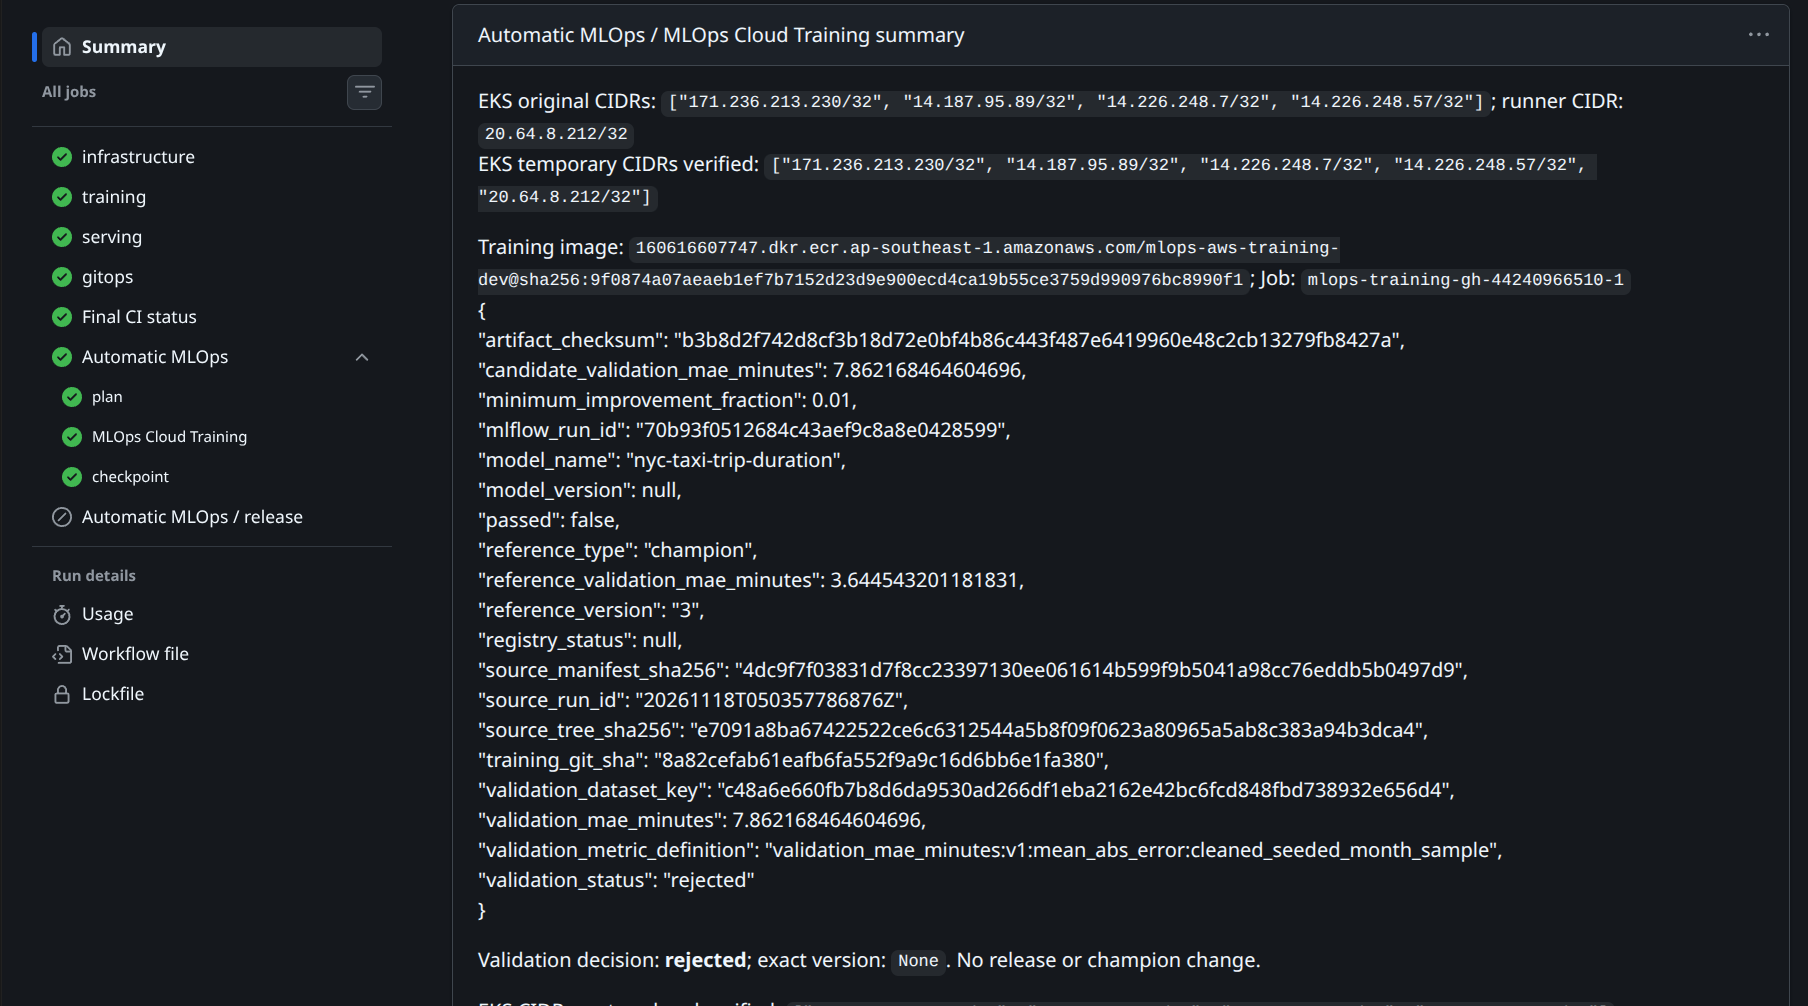
\includegraphics[width=0.94\linewidth,height=0.30\textheight,keepaspectratio,trim={450.00000bp 0.00000bp 10.00000bp 300.00000bp},clip]{Pictures/h02-rejected.png}
\caption{Candidate bị từ chối}
\end{subfigure}\par\medskip
\caption{Kết quả kiểm duyệt mô hình trong hai trường hợp Approved và Rejected.}
\label{fig:h02}
\end{figure}

\begin{table}[!htbp]\centering
\fontsize{12}{15}\selectfont\setstretch{1.05}
\setlength{\tabcolsep}{4pt}\setlength{\arrayrulewidth}{0.4pt}\renewcommand{\arraystretch}{1.2}
\setlength{\ReportTableWidth}{\dimexpr\linewidth-4\arrayrulewidth\relax}
\begin{tabular}{|L{\dimexpr 0.44\ReportTableWidth-2\tabcolsep\relax}|L{\dimexpr 0.28\ReportTableWidth-2\tabcolsep\relax}|L{\dimexpr 0.28\ReportTableWidth-2\tabcolsep\relax}|}
\hline
\textbf{Tiêu chí} & \textbf{Approved} & \textbf{Rejected} \\
\hline
Candidate MAE (phút) & 3,6445 & 7,8622 \\\hline
Reference MAE (phút) & 3,6949 & 3,6445 \\\hline
Reference model & v2 & v3 \\\hline
Validation Gate & Approved & Rejected \\\hline
Model version mới & v3 & Không tạo \\\hline
Release & Thực hiện & Bỏ qua \\\hline
\end{tabular}
\caption{So sánh kết quả Validation Gate}\label{tab:14}
\end{table}

Trong trường hợp \textbf{Approved}, mô hình ứng viên đạt MAE 3,6445 phút, cải thiện khoảng \textbf{1,36\%} so với champion v2. Kết quả vượt ngưỡng kiểm duyệt, được đăng ký thành phiên bản v3 và chuyển tiếp sang quy trình phát hành.


Ngược lại, mô hình ở trường hợp \textbf{Rejected} có MAE 7,8622 phút, không đáp ứng yêu cầu cải thiện so với champion v3. Hệ thống ghi nhận kết quả huấn luyện nhưng không tạo Registry version mới và tự động bỏ qua Release.


Đáng chú ý, Training workflow trong cả hai trường hợp đều hoàn tất thành công về mặt thực thi. Điều này cho thấy hệ thống phân biệt được \textbf{trạng thái thực thi huấn luyện} với \textbf{quyết định chất lượng mô hình}, tránh phát hành một mô hình chỉ vì quá trình huấn luyện không gặp lỗi kỹ thuật.


\FloatBarrier

\subsubsection{Kiểm chứng MLflow Model Registry}


\begin{figure}[!htbp]
\centering
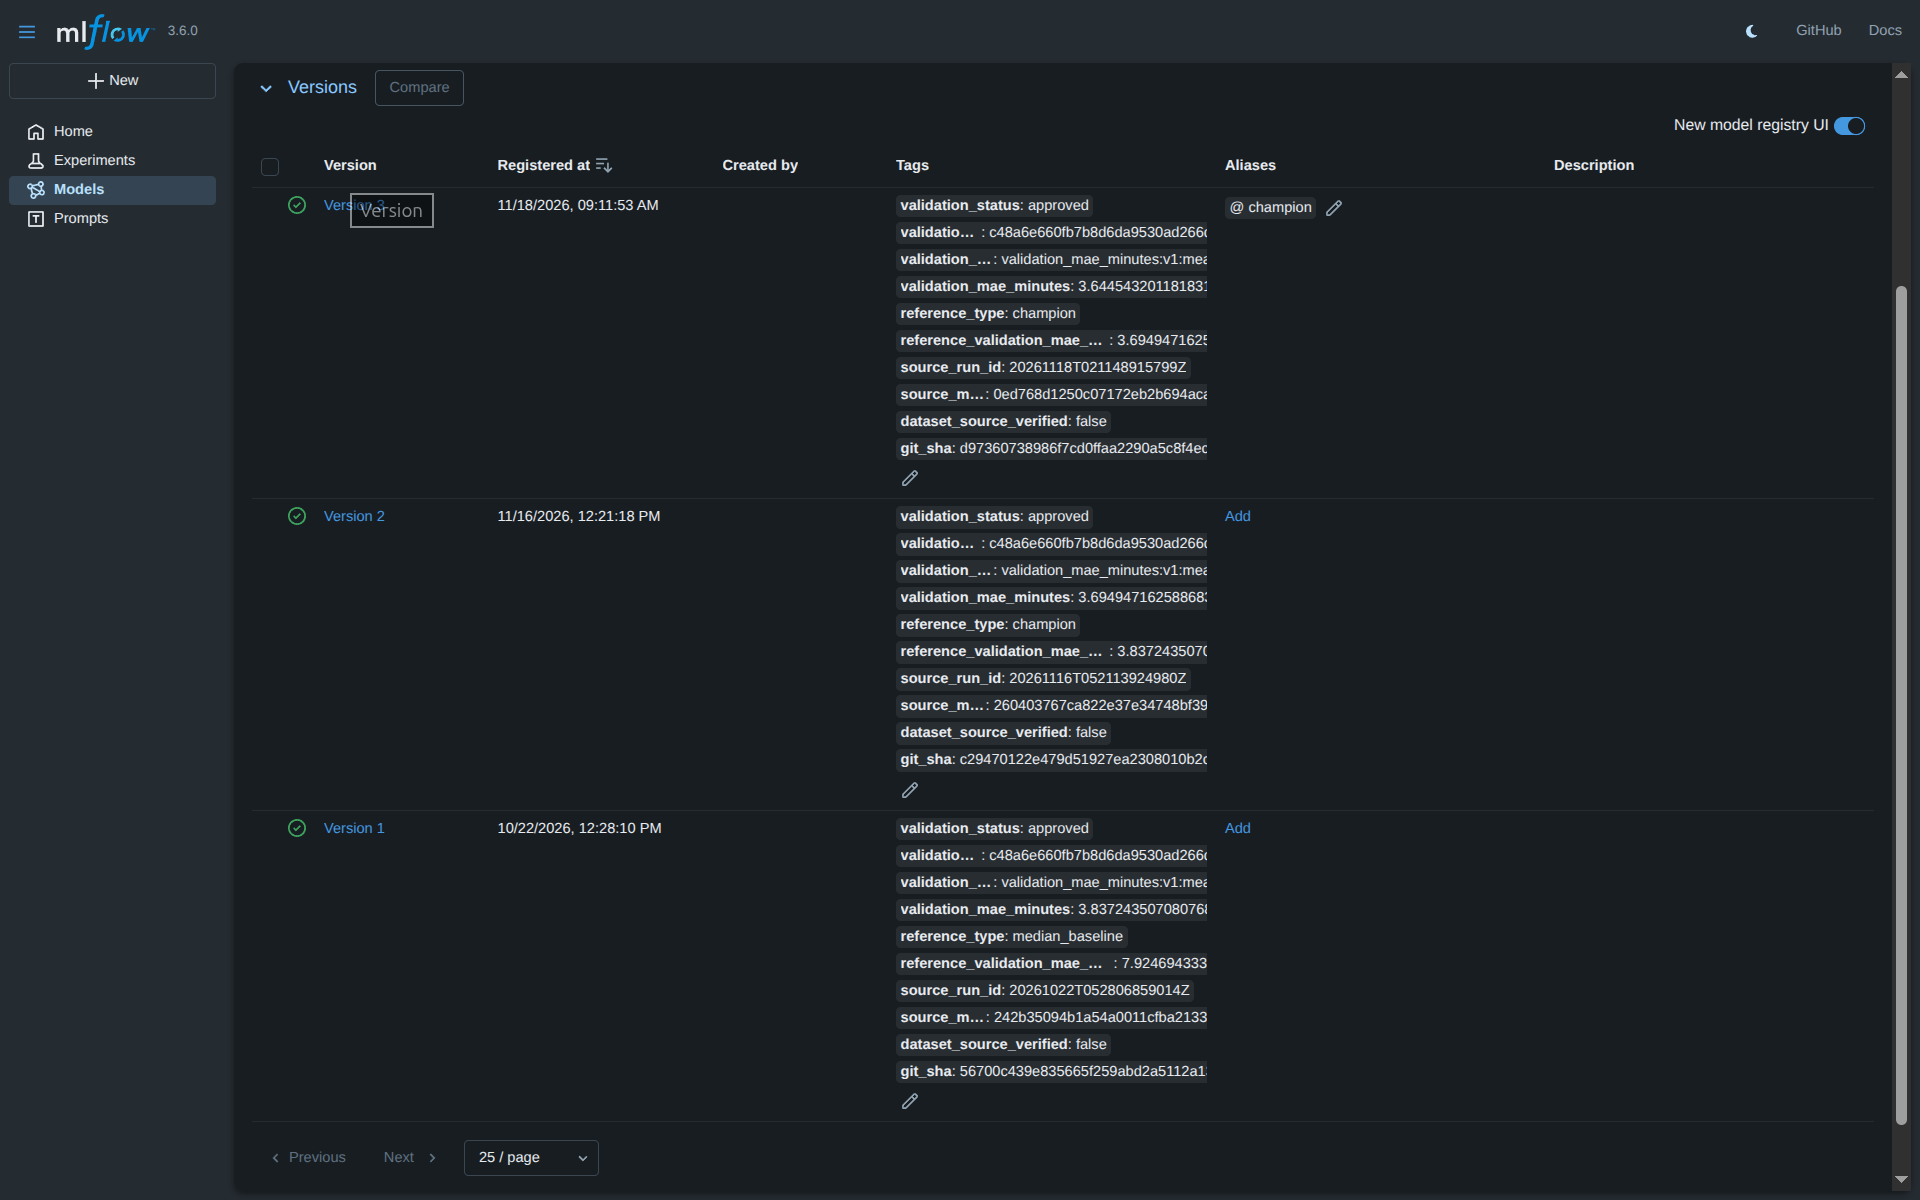
\includegraphics[width=0.94\linewidth,height=0.46\textheight,keepaspectratio,trim={250.00000bp 70.00000bp 440.00000bp 60.00000bp},clip]{Pictures/h03-registry.png}
\caption{Các phiên bản mô hình được quản lý trong MLflow Model Registry.}
\label{fig:h03}
\end{figure}

MLflow ghi nhận ba phiên bản mô hình đã được phê duyệt, với Validation MAE lần lượt là 3,8372 phút (v1), 3,6949 phút (v2) và 3,6445 phút (v3). Alias \code{champion} hiện trỏ đến v3 sau khi phiên bản này hoàn tất quá trình phát hành và xác minh dịch vụ.


Đối với mô hình bị từ chối, thông tin huấn luyện vẫn được lưu trong MLflow Tracking để phục vụ truy vết, nhưng không xuất hiện thêm phiên bản trong Registry. Kết quả cho thấy hệ thống duy trì được lịch sử thí nghiệm mà không làm ảnh hưởng đến phiên bản đang phục vụ.


\FloatBarrier

\subsection{Kiểm chứng dịch vụ suy luận và giám sát vận hành}


\subsubsection{Kiểm chứng FastAPI Model Serving}


Dịch vụ FastAPI được kiểm tra thông qua các endpoint \code{/model-info} và \code{/predict} trên môi trường EKS.


\begin{figure}[!htbp]
\centering
\begin{subfigure}{\linewidth}
\centering
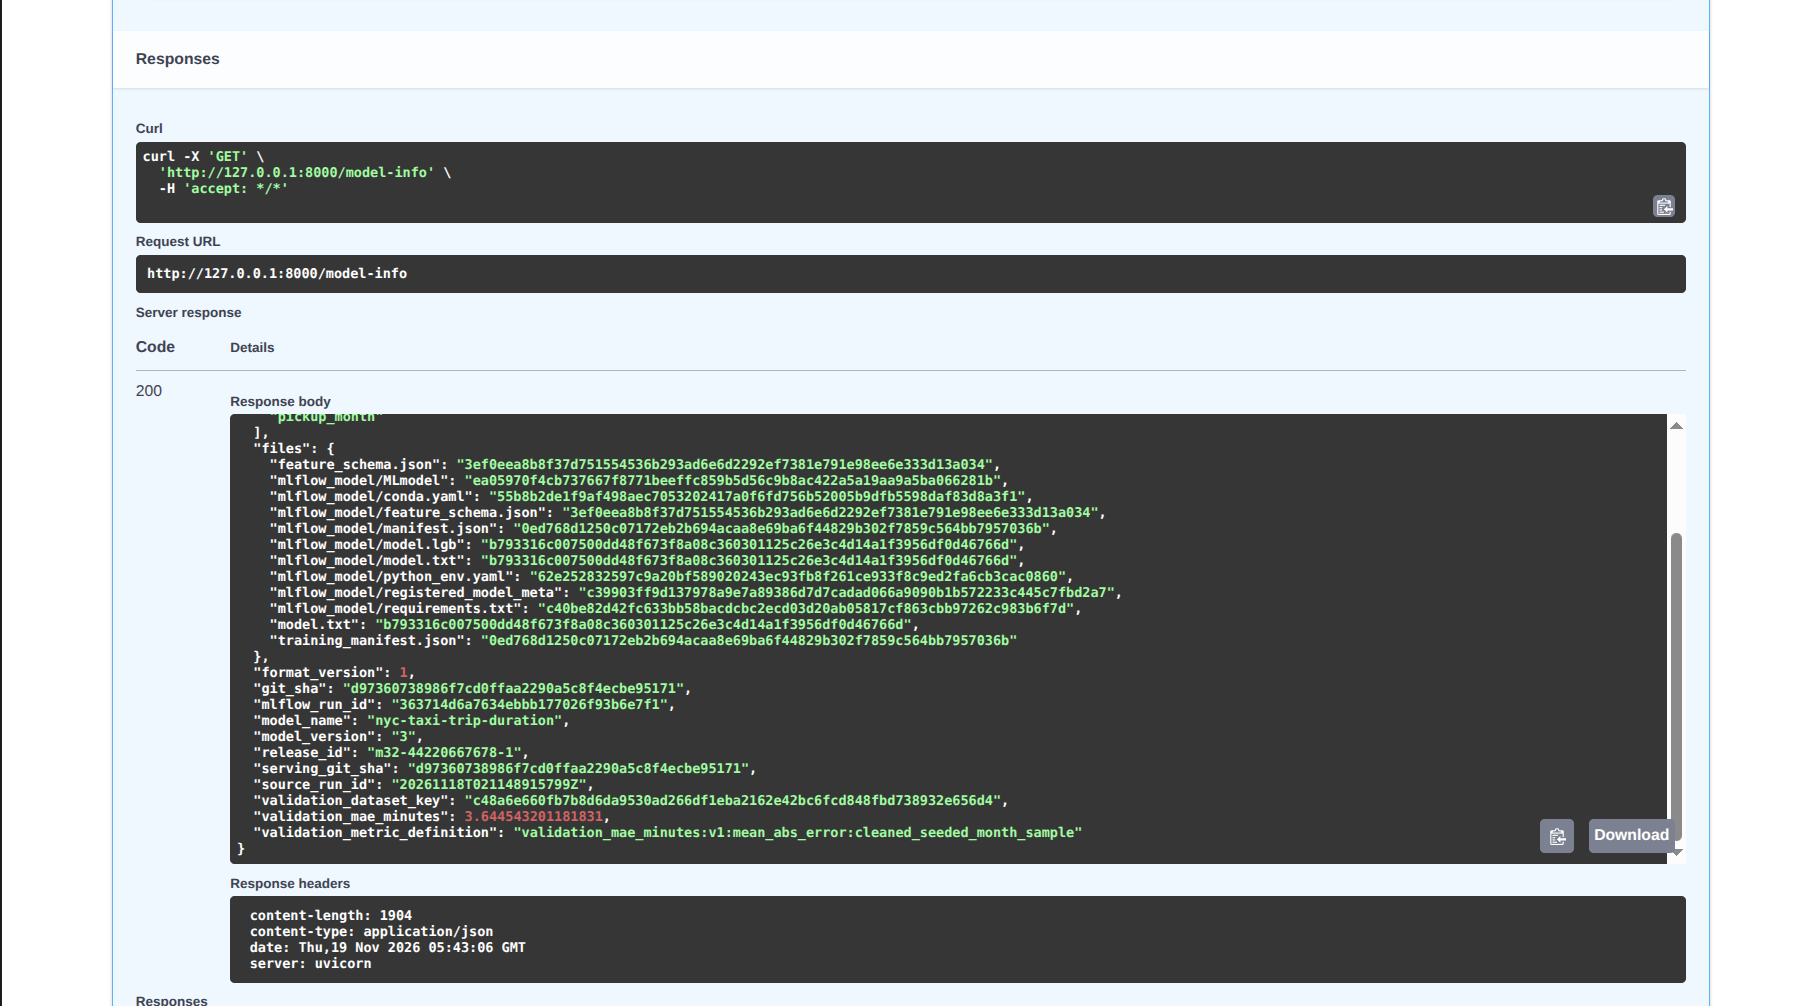
\includegraphics[width=0.94\linewidth,height=0.27\textheight,keepaspectratio,trim={112.00000bp 20.00000bp 95.00000bp 30.00000bp},clip]{Pictures/h04-model-info.png}
\caption{Thông tin mô hình đang phục vụ}
\end{subfigure}\par\medskip
\begin{subfigure}{\linewidth}
\centering
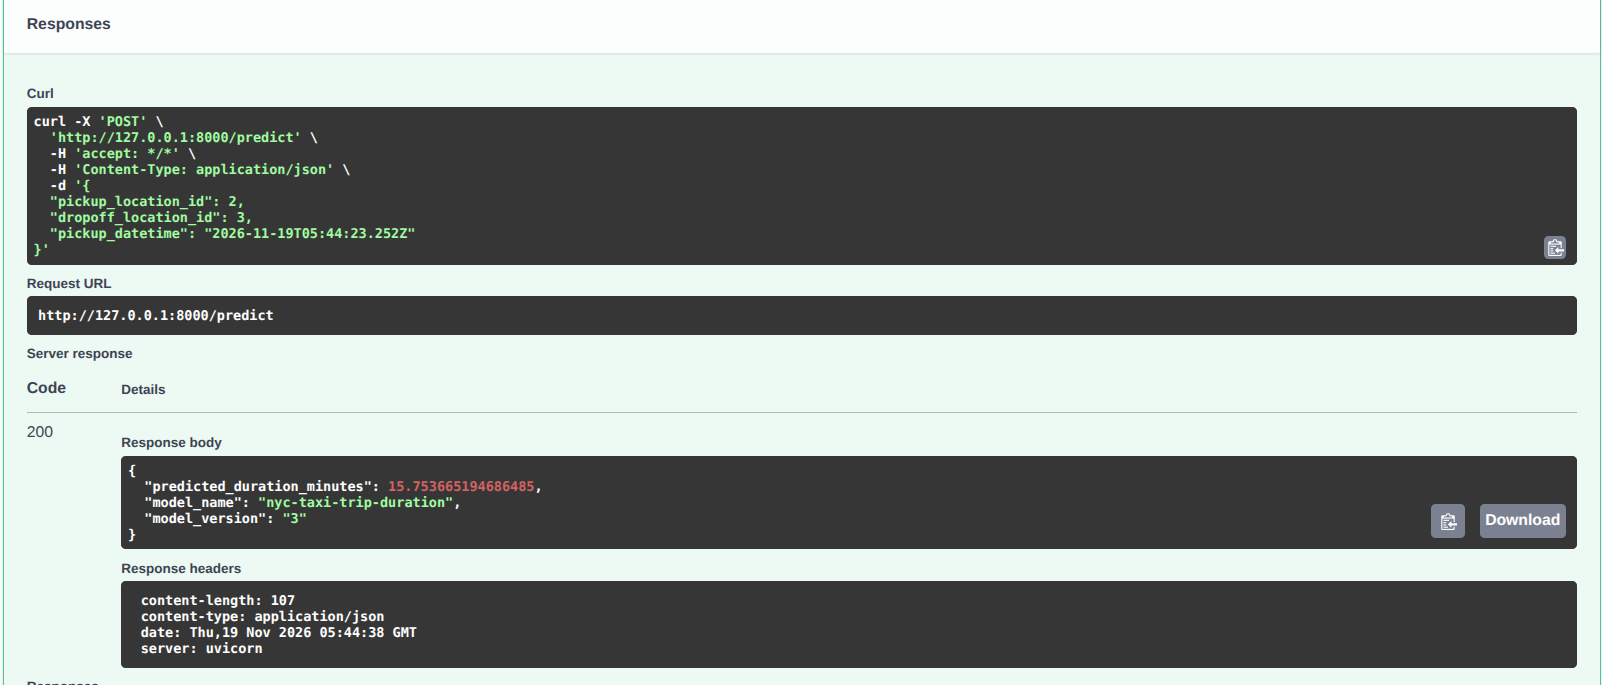
\includegraphics[width=0.94\linewidth,height=0.27\textheight,keepaspectratio]{Pictures/h04-predict.png}
\caption{Kết quả dự đoán}
\end{subfigure}\par\medskip
\caption{Kết quả truy xuất thông tin mô hình và thực hiện dự đoán qua FastAPI.}
\label{fig:h04}
\end{figure}

API \code{/model-info} trả về HTTP 200 cùng thông tin mô hình đang phục vụ, bao gồm phiên bản v3, MLflow Run ID, Release ID và các metadata kiểm chứng tương ứng.


Đối với \code{/predict}, hệ thống xử lý thành công yêu cầu dự đoán thời lượng chuyến đi và trả về kết quả \textbf{15,7537 phút}, kèm tên và phiên bản mô hình v3.


Kết quả xác nhận ứng dụng suy luận đã nạp đúng phiên bản được phát hành và có khả năng xử lý yêu cầu thực tế. Thông tin định danh được đối chiếu với MLflow Registry và gói mô hình đã triển khai nhằm bảo đảm tính nhất quán giữa huấn luyện và phục vụ.


\FloatBarrier

\subsubsection{Kiểm chứng GitOps Deployment}


\begin{figure}[!htbp]
\centering
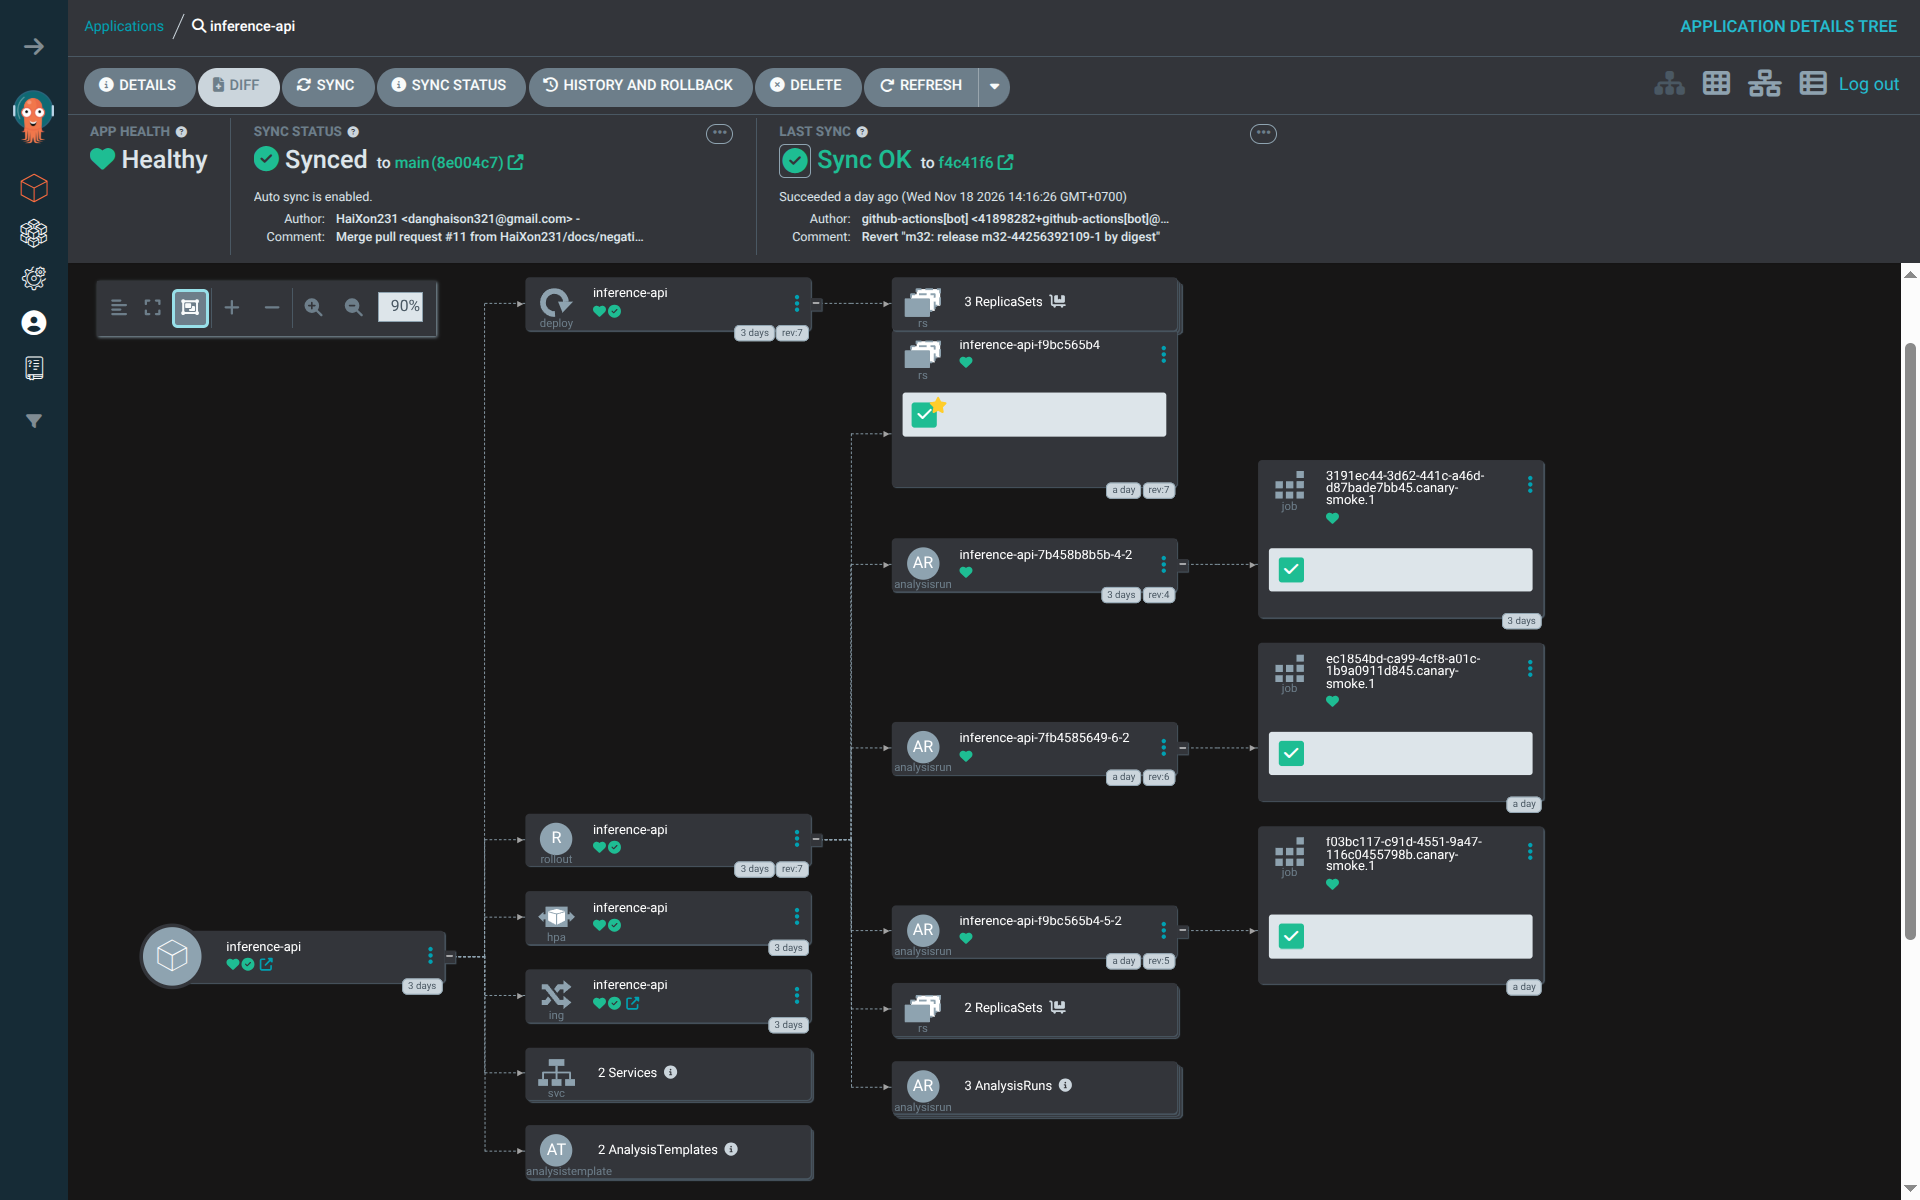
\includegraphics[width=0.94\linewidth,height=0.46\textheight,keepaspectratio]{Pictures/h05-argocd.png}
\caption{Trạng thái đồng bộ và các tài nguyên Kubernetes được quản lý bởi Argo CD.}
\label{fig:h05}
\end{figure}

Giao diện Argo CD ghi nhận Application \code{inference-api} ở trạng thái \textbf{Synced} và \textbf{Healthy}. Các tài nguyên liên quan, gồm Rollout, ReplicaSets, Services, HPA và AnalysisRuns, được quản lý trong cùng Application.


Đối chiếu trạng thái GitOps với hệ thống đang chạy cho thấy phiên bản phục vụ được đồng bộ theo cấu hình lưu trong Git. Sau các thử nghiệm phát hành và khôi phục, Argo CD tiếp tục duy trì trạng thái Healthy với mô hình champion v3.


Kết quả này xác nhận khả năng quản lý trạng thái triển khai và khôi phục cấu hình của cơ chế GitOps đã hiện thực.


\FloatBarrier

\subsubsection{Đánh giá giám sát và tự động mở rộng}


Nhóm sử dụng k6 để tạo lưu lượng HTTP qua Internal ALB nhằm đánh giá khả năng phục vụ và phản ứng của HPA khi tải thay đổi. Các chỉ số request rate được thu thập từ Prometheus, trong khi mức sử dụng CPU và số lượng replica được ghi nhận từ Kubernetes HPA. Dữ liệu lịch sử sau đó được tái hiện trên Grafana thông qua TestData CSV Content để quan sát đồng thời các chỉ số.


\begin{figure}[!htbp]
\centering
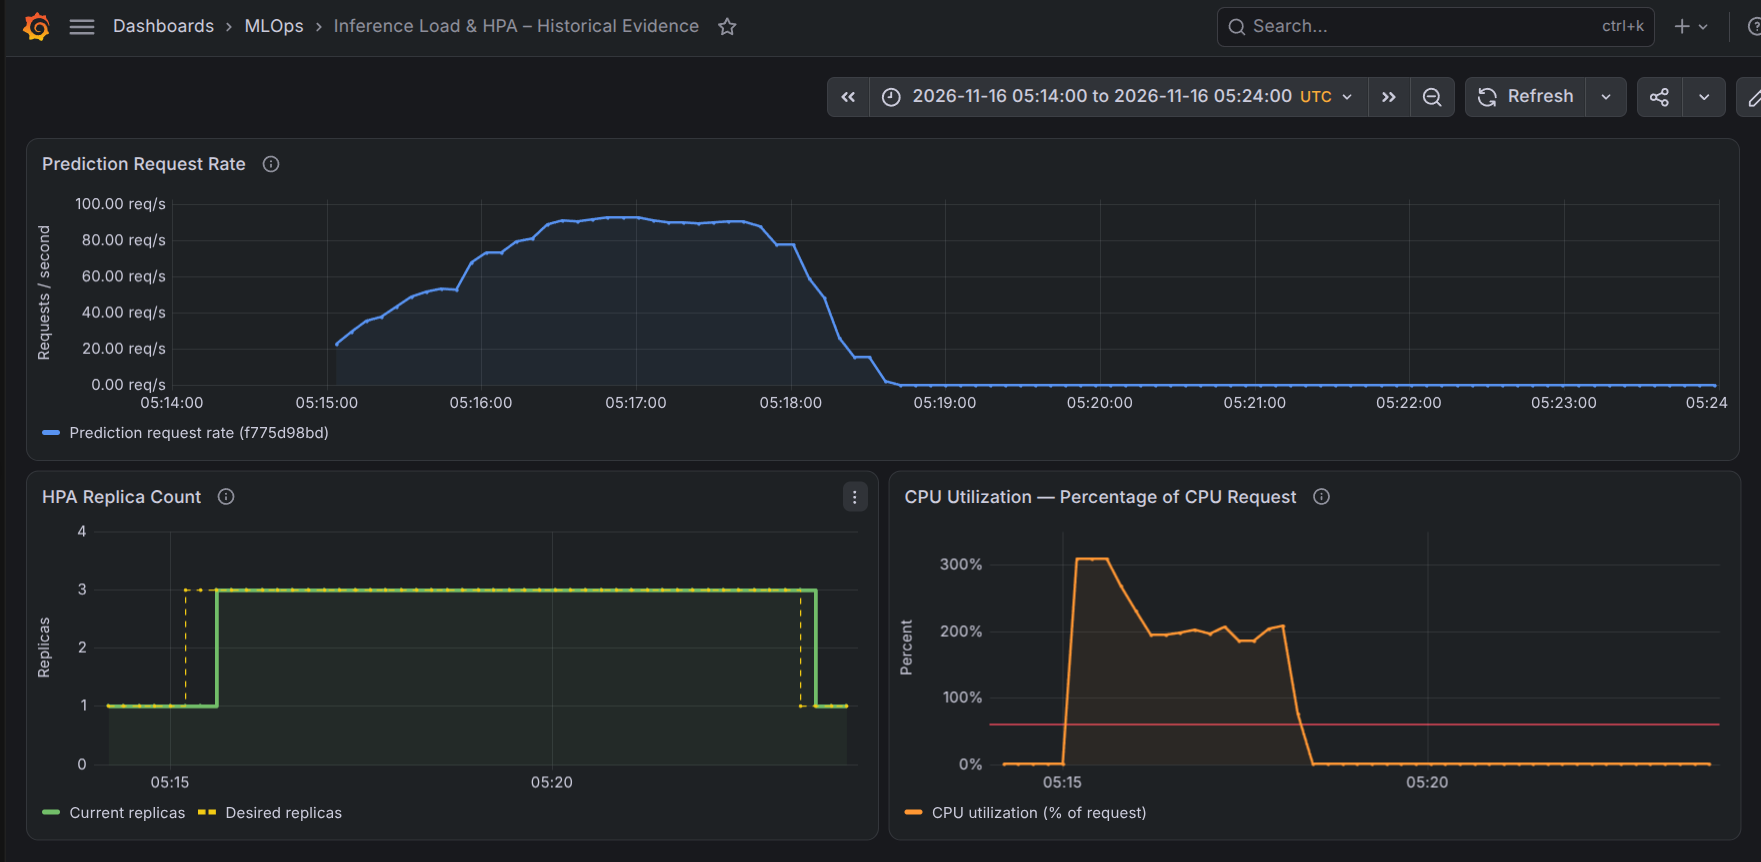
\includegraphics[width=0.94\linewidth,height=0.46\textheight,keepaspectratio]{Pictures/h06-hpa.png}
\caption{Diễn biến thông lượng yêu cầu, mức sử dụng CPU và số lượng replica trong thử nghiệm HPA.}
\label{fig:h06}
\caption*{\footnotesize Dữ liệu lịch sử được tái hiện trên Grafana bằng TestData CSV Content.}
\end{figure}

\begin{table}[!htbp]\centering
\fontsize{12}{15}\selectfont\setstretch{1.05}
\setlength{\tabcolsep}{4pt}\setlength{\arrayrulewidth}{0.4pt}\renewcommand{\arraystretch}{1.2}
\setlength{\ReportTableWidth}{\dimexpr\linewidth-4\arrayrulewidth\relax}
\begin{tabular}{|L{\dimexpr 0.42\ReportTableWidth-2\tabcolsep\relax}|L{\dimexpr 0.27\ReportTableWidth-2\tabcolsep\relax}|L{\dimexpr 0.31\ReportTableWidth-2\tabcolsep\relax}|}
\hline
\textbf{Chỉ số} & \textbf{Hiệu chỉnh tải} & \textbf{Tải phát hành thông thường} \\
\hline
Tải yêu cầu (RPS) & 100 & 40 \\\hline
Tốc độ xử lý thực tế (RPS) & 83,17 & 39,85 \\\hline
Tổng số yêu cầu hoàn thành & 14.974 & 23.913 \\\hline
P95 phía client (ms) & 603,84 & 31,63 \\\hline
HTTP failures & 4 & 0 \\\hline
Dropped iterations & 3.026 & 88 \\\hline
\end{tabular}
\caption{Kết quả các kịch bản kiểm thử tải}\label{tab:15}
\end{table}

Hai kịch bản được thực hiện độc lập: thử nghiệm hiệu chỉnh tải sử dụng phiên bản Stable v1 để quan sát HPA, trong khi tải phát hành thông thường được ghi nhận trong quá trình phát hành v1 lên v2.


Ở mức tải 40 RPS, hệ thống đạt tốc độ xử lý thực tế gần với mức yêu cầu, với P95 khoảng 31,63 ms và không ghi nhận HTTP failure trong bài kiểm thử này.


Khi tăng tải lên 100 RPS, tốc độ xử lý thực tế đạt 83,17 RPS, độ trễ P95 tăng đáng kể và xuất hiện các iterations không thể khởi tạo đúng lịch. Thử nghiệm đồng thời ghi nhận bốn phản hồi ELB 502. Kết quả cho thấy hệ thống chưa duy trì được thông lượng mục tiêu 100 RPS trong cấu hình kiểm thử này.


Biểu đồ Grafana cho thấy mức sử dụng CPU tăng vượt ngưỡng mục tiêu 60\%, có thời điểm đạt \textbf{310\% CPU request}. HPA tương ứng điều chỉnh số lượng replica từ \textbf{1 lên 3}, sau đó giảm về \textbf{1} khi tải kết thúc và hết thời gian ổn định. Diễn biến này xác nhận HPA đã phản ứng với sự thay đổi tải và điều chỉnh số lượng Pod theo cấu hình.


Những kết quả trên xác nhận cơ chế giám sát và tự động mở rộng hoạt động theo thiết kế. Tuy nhiên, thí nghiệm chưa có đối chứng cùng mức tải với số replica cố định, nên chưa kết luận mức cải thiện throughput do riêng HPA mang lại.


\FloatBarrier

\subsection{Kiểm chứng Canary Deployment và tự động hóa toàn trình}


\subsubsection{Kiểm chứng Canary thất bại và tự động khôi phục}


Để đánh giá khả năng xử lý phiên bản không đạt yêu cầu, nhóm thực hiện một Release có kiểm soát trên mô hình v3. Phiên bản Stable giữ nguyên cấu hình, trong khi Canary candidate sử dụng cùng mô hình nhưng bị giới hạn CPU xuống \code{100m} nhằm tạo ra sự suy giảm hiệu năng khi nhận lưu lượng.


Smoke Test ban đầu thành công, xác nhận candidate có thể khởi động và thực hiện suy luận. Tuy nhiên, khi nhận lưu lượng thực, AnalysisRun ghi nhận hai mẫu P95 lần lượt là \textbf{964,31 ms} và \textbf{884,37 ms}, vượt ngưỡng cho phép 500 ms.


Các tiêu chí về tốc độ yêu cầu và tỷ lệ lỗi HTTP 5xx tại ứng dụng vẫn đạt yêu cầu. Vì vậy, quyết định từ chối Canary xuất phát từ vi phạm điều kiện độ trễ, không phải lỗi khởi động hoặc thiếu lưu lượng đánh giá.


\begin{figure}[!htbp]
\centering
\begin{subfigure}{\linewidth}
\centering
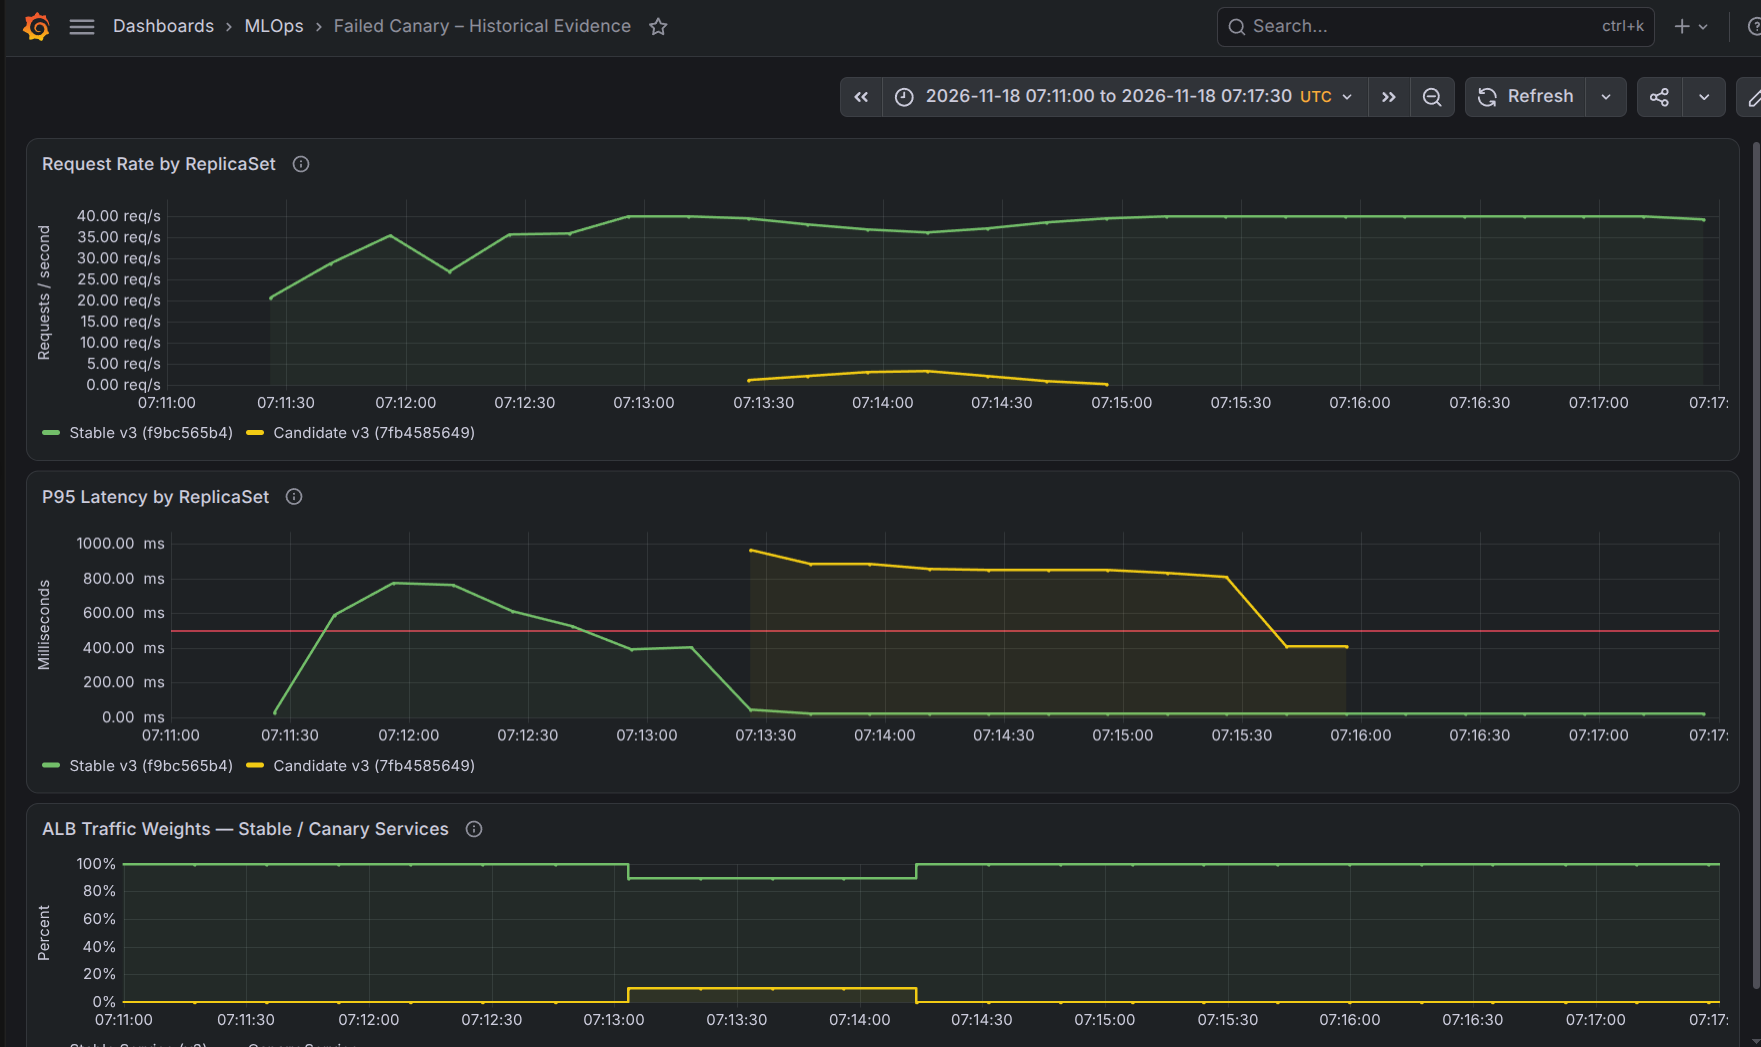
\includegraphics[width=0.94\linewidth,height=0.40\textheight,keepaspectratio]{Pictures/h07-failed-canary.png}
\caption{Diễn biến Canary thất bại và khôi phục lưu lượng về Stable}
\end{subfigure}\par\medskip
\begin{subfigure}{\linewidth}
\centering
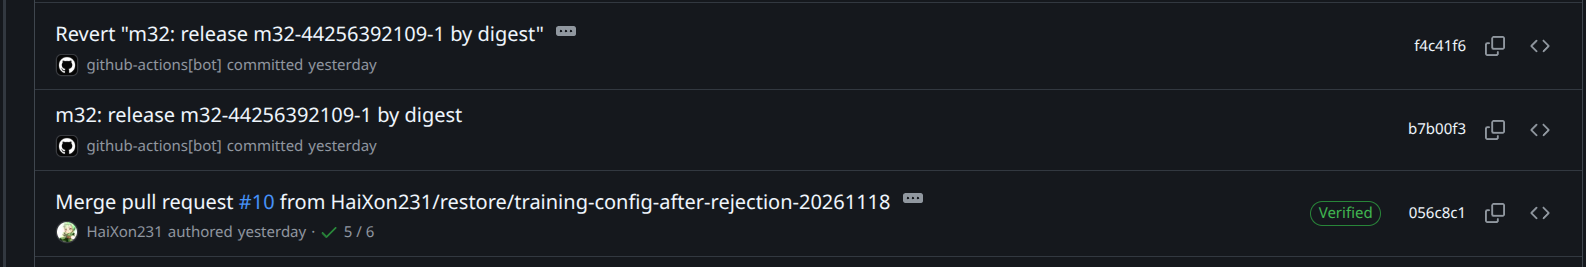
\includegraphics[width=0.94\linewidth,height=0.12\textheight,keepaspectratio,trim={0.00000bp 97.00000bp 0.00000bp 0.00000bp},clip]{Pictures/h07-git-revert.png}
\caption{Git revert commit do GitHub Actions tạo để hoàn tác Release}
\end{subfigure}\par\medskip
\caption{Biến động thông lượng, độ trễ P95 và phân phối lưu lượng ALB khi Canary bị từ chối.}
\label{fig:h07}
\caption*{\footnotesize Dữ liệu lịch sử được tái hiện trên Grafana bằng TestData CSV Content.}
\end{figure}

Biểu đồ Grafana cho thấy Canary vẫn tiếp nhận yêu cầu tại bước phân phối 10\%, nhưng độ trễ P95 tăng vượt ngưỡng kiểm duyệt. Khi AnalysisRun chuyển sang trạng thái Failed, Argo Rollouts thực hiện \textbf{Abort}, đưa lưu lượng trở lại Stable. Release workflow sau đó tự động tạo Git revert commit để hoàn tác cấu hình triển khai ứng viên.


Kết quả xác minh sau khôi phục cho thấy:


\begin{itemize}

\item 

Argo CD trở về trạng thái Synced/Healthy.


\item 

Stable sử dụng lại image và cấu hình CPU ban đầu.


\item 

MLflow champion và phiên bản đang phục vụ vẫn là v3.


\end{itemize}

Thử nghiệm xác nhận hệ thống có khả năng từ chối một Canary vi phạm điều kiện hiệu năng và khôi phục trạng thái triển khai đã được xác minh. Trường hợp này sử dụng Release workflow được kích hoạt thủ công với cơ chế fault injection, không phải một lần chạy đầy đủ toàn bộ pipeline tự động.


\FloatBarrier

\subsubsection{Kiểm chứng Canary thành công}


Trong trường hợp phát hành thành công, hệ thống thực hiện chuyển đổi từ mô hình v2 sang v3 thông qua các giai đoạn phân phối lưu lượng tăng dần. Candidate được đánh giá bằng Prometheus trong quá trình triển khai trước khi hoàn tất Promotion và trở thành phiên bản Stable mới.


\begin{figure}[!htbp]
\centering
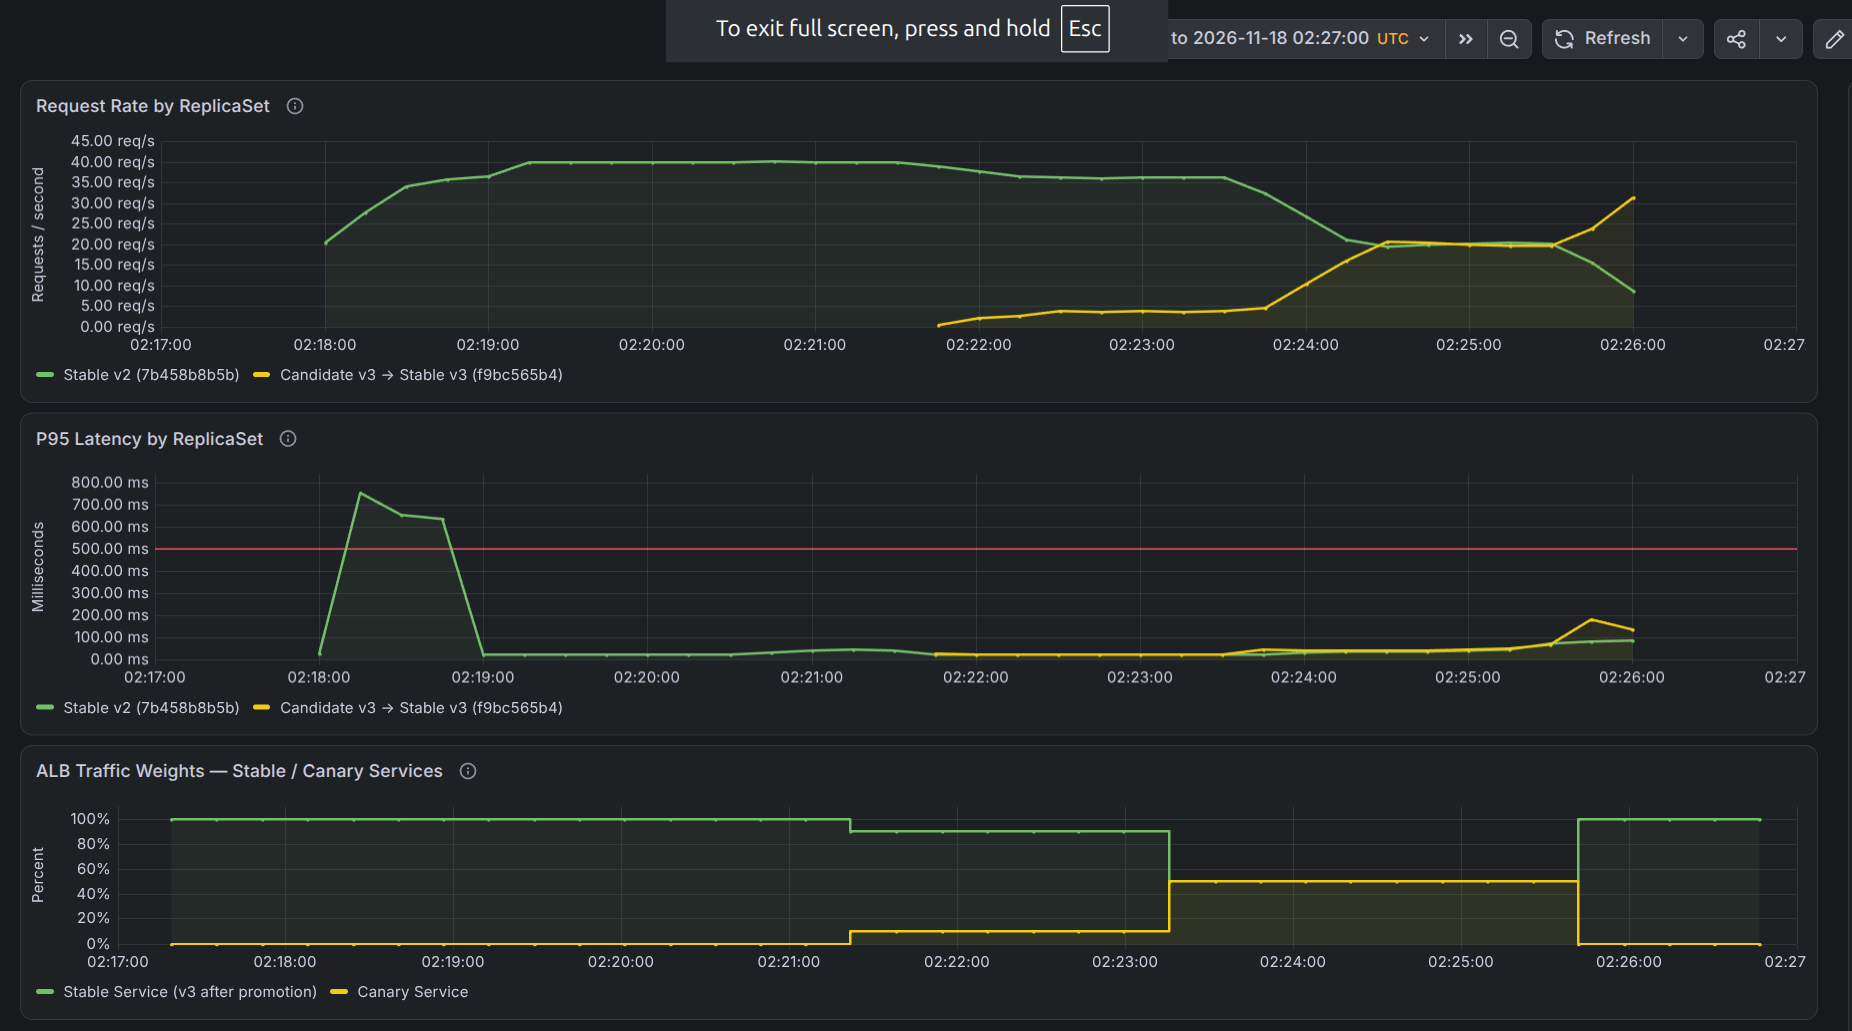
\includegraphics[width=0.94\linewidth,height=0.46\textheight,keepaspectratio,trim={0.00000bp 0.00000bp 0.00000bp 70.00000bp},clip]{Pictures/h08-successful-canary.png}
\caption{Thông lượng, độ trễ P95 và quá trình chuyển đổi lưu lượng khi Canary v3 được phát hành thành công.}
\label{fig:h08}
\caption*{\footnotesize Dữ liệu lịch sử được tái hiện trên Grafana bằng TestData CSV Content.}
\end{figure}

Kết quả quan sát trực tiếp từ ALB xác nhận các trạng thái phân bổ lưu lượng:


\begin{table}[!htbp]\centering
\fontsize{12}{15}\selectfont\setstretch{1.05}
\setlength{\tabcolsep}{4pt}\setlength{\arrayrulewidth}{0.4pt}\renewcommand{\arraystretch}{1.2}
\setlength{\ReportTableWidth}{\dimexpr\linewidth-4\arrayrulewidth\relax}
\begin{tabular}{|L{\dimexpr 0.5\ReportTableWidth-2\tabcolsep\relax}|L{\dimexpr 0.25\ReportTableWidth-2\tabcolsep\relax}|L{\dimexpr 0.25\ReportTableWidth-2\tabcolsep\relax}|}
\hline
\textbf{Giai đoạn} & \textbf{Stable} & \textbf{Canary} \\
\hline
Ban đầu & 100\% & 0\% \\\hline
Canary bước 1 & 90\% & 10\% \\\hline
Canary bước 2 & 50\% & 50\% \\\hline
Sau Promotion & 100\% & 0\% \\\hline
\end{tabular}
\caption{Phân bổ lưu lượng trong quá trình phát hành thành công}\label{tab:16}
\end{table}

Biểu đồ Grafana thể hiện sự thay đổi request rate giữa hai ReplicaSet tương ứng với quá trình chuyển đổi lưu lượng. Các số liệu Prometheus cho thấy tỷ lệ lưu lượng đến Canary ước lượng khoảng \textbf{9,59\%} và \textbf{49,83\%} tại hai bước kiểm thử, phù hợp với trọng số định tuyến được cấu hình.


Trong các mẫu đánh giá hợp lệ của AnalysisRun, Canary đạt toàn bộ điều kiện kiểm duyệt. P95 phía server dao động khoảng 24,56–46,67 ms, thấp hơn ngưỡng 500 ms; tỷ lệ lỗi HTTP 5xx của ứng dụng bằng 0. Những mẫu chưa đủ dữ liệu ban đầu được đánh giá lại khi lưu lượng trở nên phù hợp.


Sau khi Canary thành công, hệ thống xác minh trạng thái phục vụ trước khi cập nhật \code{champion} từ v2 sang v3. Trọng số 100/0 ở bước cuối tương ứng với Stable đã chuyển sang mô hình mới, không phải khôi phục phiên bản cũ.


\FloatBarrier

\subsubsection{Kiểm chứng quy trình MLOps tự động toàn trình}


\begin{figure}[!htbp]
\centering
\begin{subfigure}{\linewidth}
\centering
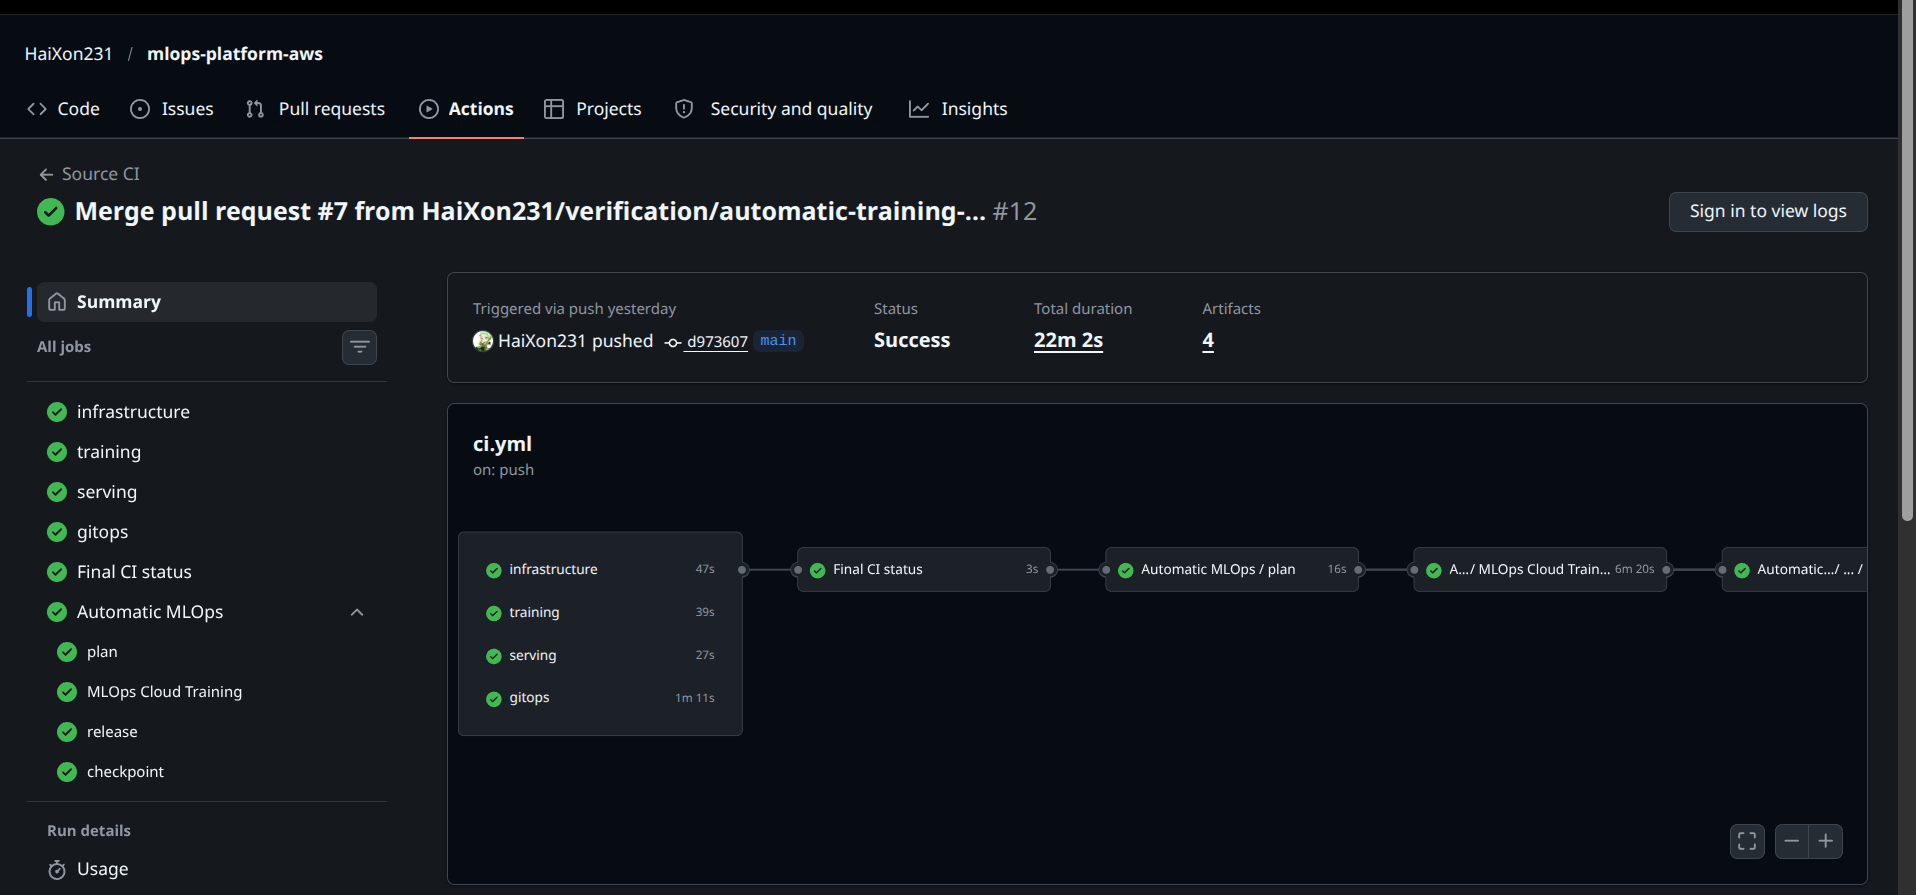
\includegraphics[width=0.94\linewidth,height=0.30\textheight,keepaspectratio]{Pictures/h09-pipeline.png}
\caption{Các jobs của pipeline tự động}
\end{subfigure}\par\medskip
\begin{subfigure}{\linewidth}
\centering
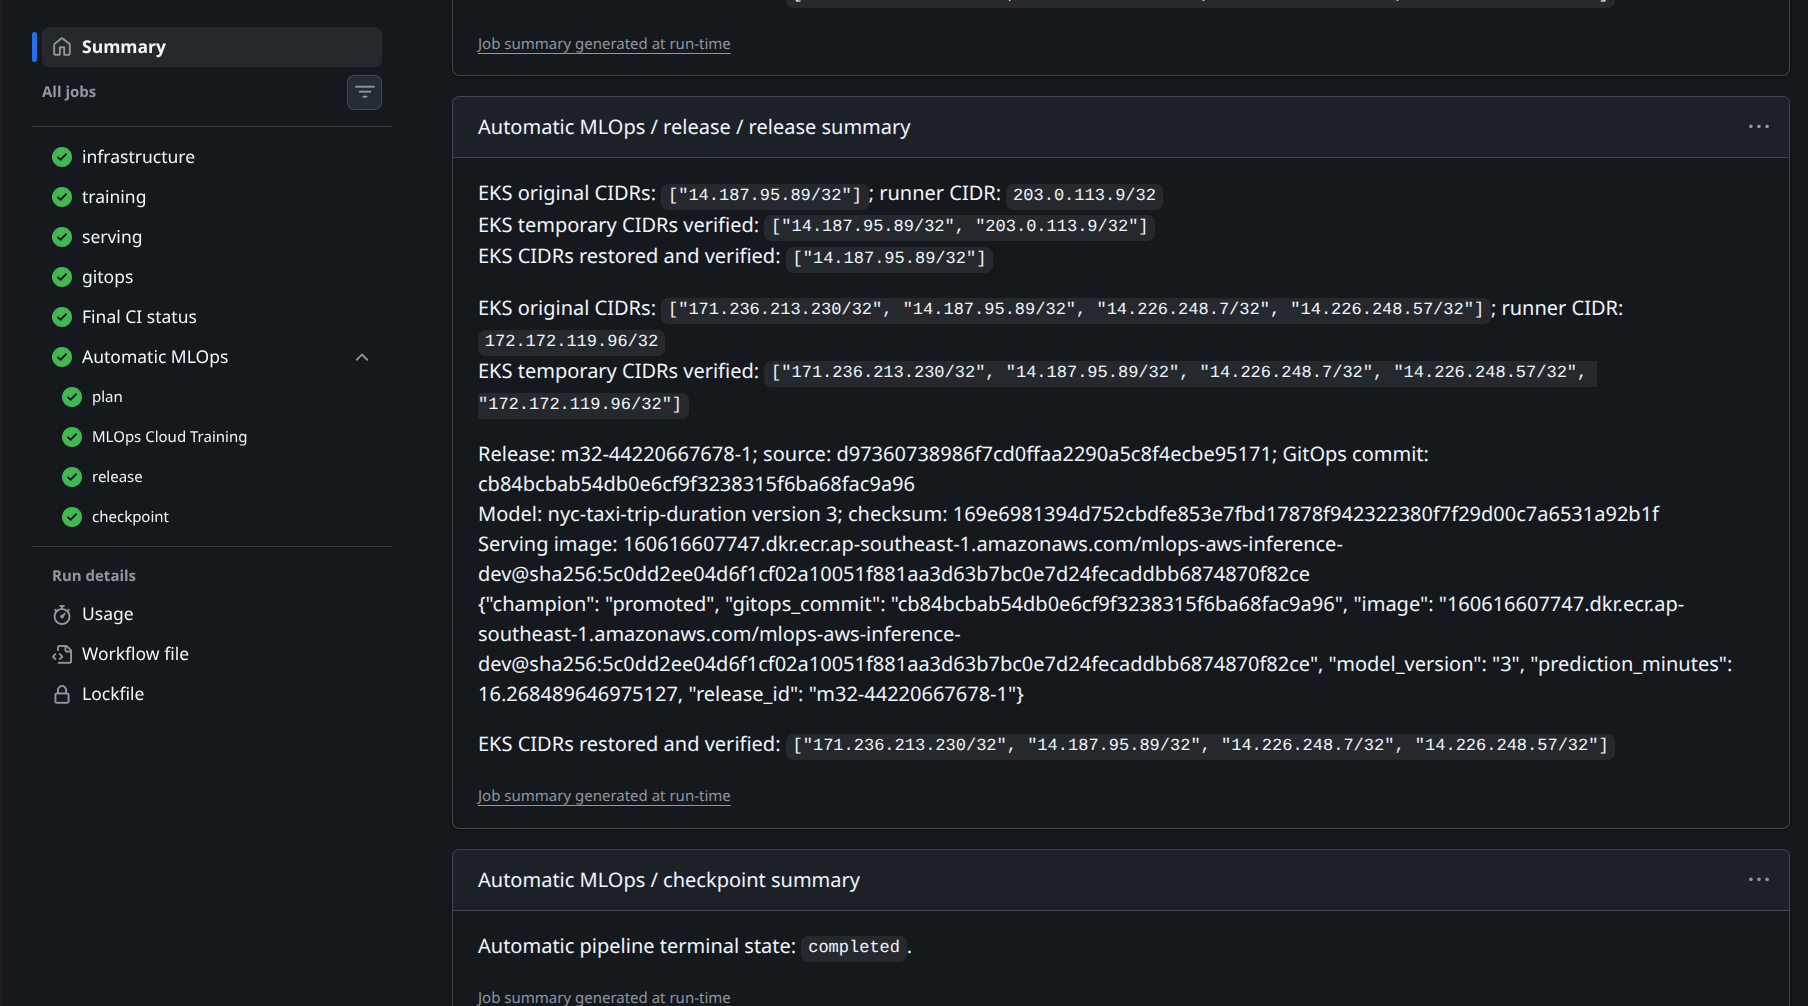
\includegraphics[width=0.94\linewidth,height=0.30\textheight,keepaspectratio,trim={460.00000bp 0.00000bp 20.00000bp 55.00000bp},clip]{Pictures/h09-completed.png}
\caption{Kết quả Release và checkpoint completed}
\end{subfigure}\par\medskip
\caption{Kết quả thực thi tự động toàn bộ quy trình CI, Training và Release trên GitHub Actions.}
\label{fig:h09}
\end{figure}

Thử nghiệm end-to-end được kích hoạt từ thay đổi mã nguồn huấn luyện trên nhánh \code{main}. GitHub Actions thực hiện thành công bốn nhóm kiểm thử Infrastructure, Training, Serving và GitOps, trước khi tự động khởi chạy Training trên EKS Spot.


Khi mô hình v3 vượt Validation Gate, hệ thống tiếp tục thực hiện Release, triển khai Canary và xác minh dịch vụ mà không yêu cầu kích hoạt Training hoặc Release thủ công. Workflow ghi nhận \textbf{9/9 jobs thành công}, với checkpoint cuối ở trạng thái \code{completed}.


Kết quả đối chiếu sau khi hoàn tất cho thấy mô hình được phê duyệt, phiên bản đang phục vụ và alias \code{champion} đều thống nhất tại v3. Hệ thống đồng thời thu hồi các Training Jobs, traffic Jobs và Spot resources tạm, trong khi các dịch vụ chính tiếp tục hoạt động.


Kết quả này chứng minh chuỗi tự động hóa \textbf{CI → Training → Validation → Release → Canary → Promotion} đã được thực thi thành công trên môi trường AWS thực tế.


\FloatBarrier

\subsubsection{Đánh giá tổng hợp}


Các thí nghiệm cho thấy nền tảng đã đáp ứng những mục tiêu chính của đề tài, từ triển khai hạ tầng, huấn luyện và quản lý mô hình đến tự động hóa phát hành và giám sát vận hành trên AWS.


Hệ thống đã kiểm chứng thành công hai lớp kiểm soát chất lượng. \textbf{Validation Gate} chỉ chấp thuận những mô hình đạt yêu cầu, trong khi \textbf{Canary Analysis} đánh giá khả năng vận hành trước khi phát hành. Các thử nghiệm xác nhận cả hai trường hợp: phiên bản đạt yêu cầu được Promotion thành công và phiên bản vi phạm điều kiện hiệu năng bị từ chối, sau đó tự động khôi phục trạng thái Stable.


Bên cạnh đó, quy trình MLOps tự động toàn trình đã được thực thi thành công, kết hợp với khả năng giám sát và điều chỉnh số lượng replica thông qua HPA. Tuy nhiên, các cơ chế mở rộng và khôi phục mới được kiểm chứng trong phạm vi thử nghiệm có kiểm soát, chưa đủ để khẳng định khả năng vận hành ổn định trong mọi tình huống.


Nhìn chung, hệ thống đã chứng minh được tính khả thi của việc tích hợp các công nghệ MLOps thành một nền tảng thống nhất, đồng thời tạo cơ sở cho những cải tiến về độ tin cậy và khả năng vận hành thực tế.

